\documentclass[border=1pt,tikz,varwidth=\maxdimen]{standalone}

\usetikzlibrary{positioning,calc,arrows}

\usepackage{amsmath,mathtools}

\begin{document}
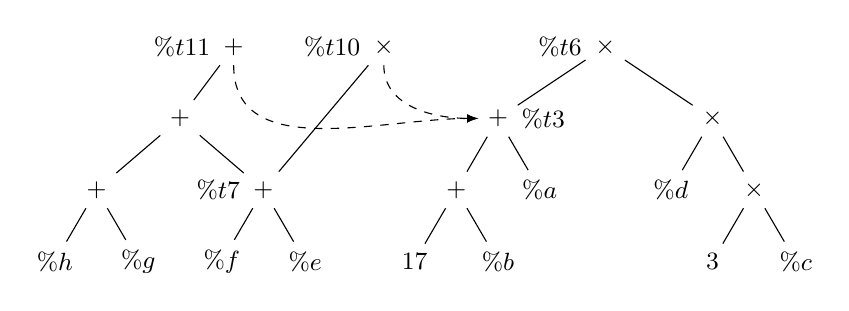
\begin{tikzpicture}[
  every node/.style={font=\small},
  level 1/.style={edge from parent,sibling distance=9ex,level distance=6ex},
  level 2/.style={edge from parent,sibling distance=7ex,level distance=6ex},
  dash-emph/.style={draw,dashed,-latex},
  empty/.style={edge from parent/.style={}},
  ]

  \node (var11-tree-root) {\(+\)}
  child {
    node {\(+\)}
    child {
      node {\(+\)}
      child {
        node {\(\%h\)}
      }
      child {
        node {\(\%g\)}
      }
    }
    child [empty] {}
    child {
      node (var7-tree-root) {\(+\)}
      child {
        node {\(\%f\)}
      }
      child {
        node {\(\%e\)}
      }
    }
  }
  child [empty] {};
  \node [left=-0.5ex of var11-tree-root] (var11-text-node) {\(\%t11\)};
  \node [left=-0.5ex of var7-tree-root] (var7-text-node) {\(\%t7\)};

  \node [right=4em of var11-tree-root] (var10-tree-root) {\(\times\)};
  \node [left=-0.5ex of var10-tree-root] (var10-text-node) {\(\%t10\)};
  \draw [solid] (var10-tree-root) -- (var7-tree-root);

  \node [right=12em of var11-tree-root] (var6-tree-root) {\(\times\)}
  child {
    node (var3-tree-root) {\(+\)}
    child {
      node {\(+\)}
      child {
        node {\(17\)}
      }
      child {
        node {\(\%b\)}
      }
    }
    child {
      node {\(\%a\)}
    }
  }
  child [empty] {}
  child {
    node {\(\times\)}
    child {
      node {\(\%d\)}
    }
    child {
      node {\(\times\)}
      child {
        node {\(3\)}
      }
      child {
        node {\(\%c\)}
      }
    }
  };
  \node [left=-0.5ex of var6-tree-root] (var6-text-node) {\(\%t6\)};
  \node [right=-0.5ex of var3-tree-root] (var3-text-node) {\(\%t3\)};

  \draw [dash-emph] (var11-tree-root) to [out=270,in=180] (var3-tree-root);
  \draw [dash-emph] (var10-tree-root) to [out=270,in=180] (var3-tree-root);

\end{tikzpicture}
\end{document}
